\def\mySecNum{10.2}
\mySection{\mySecNum~Constructing a Binomial tree}
%-------------- start slide -------------------------------%{{{ 1
\begin{frame}[fragile]
\begin{align*}
	\textcolor{magenta}{u} & = e^{(r-\delta)h \textcolor{magenta}{+} \sigma \sqrt{h}} \\
	\textcolor{cyan}{d}    & = e^{(r-\delta)h \textcolor{cyan}{-} \sigma \sqrt{h}}
\end{align*}
\bigskip
\begin{center}
	\begin{minipage}{0.72\textwidth}
		\begin{itemize}
			\item $r$: continuously compounded annual interest rate.
			\item $\delta$: continuously dividend yield.
			\item $\sigma$: annual volatility.
			\item $h$: the length of a binomial period in years.
		\end{itemize}
	\end{minipage}
\end{center}
\end{frame}
%-------------- end slide -------------------------------%}}}
%-------------- start slide -------------------------------%{{{ 1
\begin{frame}[fragile,t]
	\frametitle{Continuously Compounded Returns}
\begin{align*}
	r_{t,t+h} = \ln\left(S_{t_h}/S_t\right)
\end{align*}
\begin{align*}
	S_{t+h} = S_t e^{r_{t,t+h}}
\end{align*}
\begin{align*}
	r_{t,t+nh} = \sum_{i=1}^n r_{t+(i-1)h,t+ih}
\end{align*}
\mySeparateLine
\bigskip

\begin{center}
	\textcolor{gray}{Go over 3 examples on p. 301}
\end{center}

\end{frame}
%-------------- end slide -------------------------------%}}}
%-------------- start slide -------------------------------%{{{ 1
\begin{frame}[fragile,t]
	\frametitle{Volatility}
	The \textcolor{magenta}{volatility}	of an asset is the standard deviation of continuously
	compounded returns.
	\bigskip

	\begin{itemize}
		\item A year is dividend  into $n$ periods (say,  $n=12$) of length $h=1/n$.
		\item Let $\sigma^2$ be the annual continuously compounded return.
		\item Assuming that the continuously compounded returns are independent and identically
			distributed
		\item We have
			 \begin{align*}
				 \sigma^2 = 12 \times \sigma^2_{\text{monthly}}
			\end{align*}
			and
			\begin{align*}
				\sigma_h = \sigma \sqrt{h} \quad \text{or} \quad \sigma= \frac{\sigma_h}{\sqrt{h}}.
			\end{align*}
	\end{itemize}
\end{frame}
%-------------- end slide -------------------------------%}}}
%-------------- start slide -------------------------------%{{{ 1
\begin{frame}[fragile,t]
	\frametitle{Constructing $u$ and $d$}
	\begin{center}
		With no volatility
		\begin{align*}
			S_{t+h} = F_{t,t+h} = S_t e^{(r-\delta)h}
		\end{align*}

		\mySeparateLine

		With volatility
		\begin{align*}
			u S_t &= F_{t,t+h} e^{+\sigma \sqrt{h}} \\
			d S_t &= F_{t,t+h} e^{-\sigma \sqrt{h}}
		\end{align*}
		\begin{align*}
			\Downarrow
		\end{align*}
		\begin{align*}
			\textcolor{magenta}{u} & = e^{(r-\delta)h \textcolor{magenta}{+} \sigma \sqrt{h}} \\
			\textcolor{cyan}{d}    & = e^{(r-\delta)h \textcolor{cyan}{-} \sigma \sqrt{h}}
		\end{align*}
	\end{center}
\end{frame}
%-------------- end slide -------------------------------%}}}
%-------------- start slide -------------------------------%{{{ 1
\begin{frame}[fragile,t]
	\frametitle{Estimating Historical Volatility}
\begin{center}
	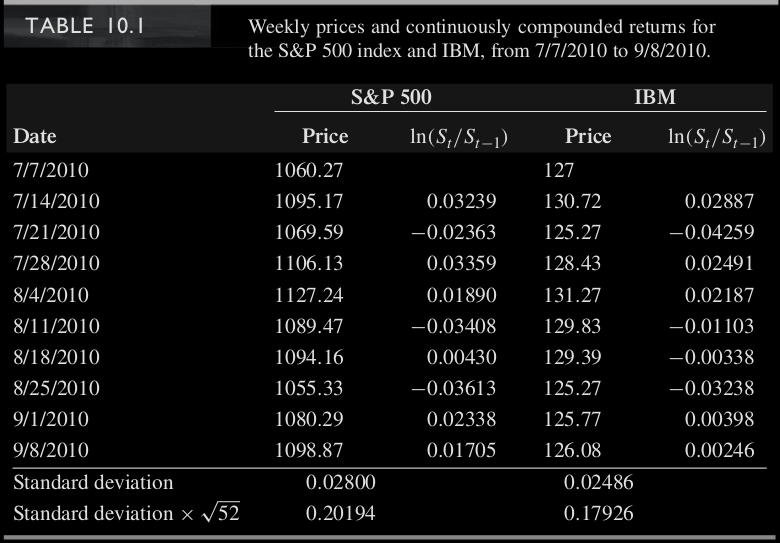
\includegraphics[scale=0.25]{figs/Table-10-1.png}
	\vfill

	\begin{itemize}
		\item Volatility computation should exclude dividend.
		\item But since dividends are small and infrequent; the standard deviation will be similar
			whether you exclude dividends or not when computing the standard deviation.
	\end{itemize}
\end{center}
\end{frame}
%-------------- end slide -------------------------------%}}}
%-------------- start slide -------------------------------%{{{ 1
\begin{frame}[fragile,t]
	\frametitle{One-period Example with a Forward Tree}
\begin{myexample}
	Consider a European call option on a stock, with a \$40 strike and 1 year to expiration. The stock
	does not pay dividends, and its current price is \$41. Suppose the volatility of the stock is
	30\%. The continuously compounded risk-free interest rate is 8\%.
	\begin{enumerate}
		\item[] Use these inputs to calculate the followings:
		\item the final stock prices $uS$ and $dS$
		\item the final option values $C_u$ and $C_d$
		\item $\Delta$ and $B$
		\item the option price: $\Delta S+B$.
	\end{enumerate}
\end{myexample}
\end{frame}
%-------------- end slide -------------------------------%}}}
%-------------- start slide -------------------------------%{{{ 1
\begin{frame}[fragile,t]
\begin{mysol}
	In summary:
	\begin{center}

	  $S=41$, $K=40$, $r=0.08$, $\delta=0$, $\sigma=0.30$, $h=1$.
		\vfill
		\pause
		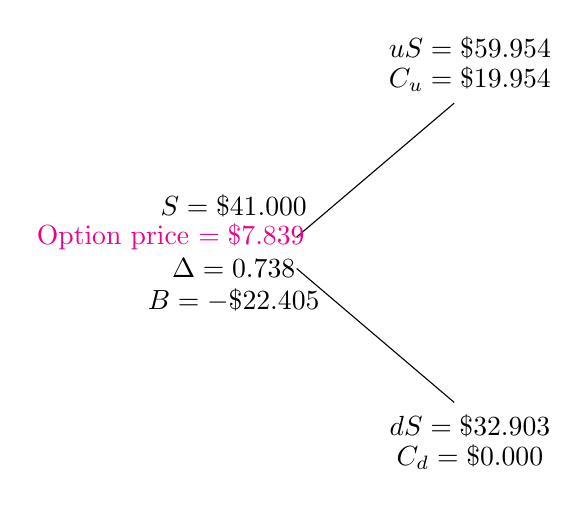
\begin{tikzpicture}[scale=1, transform shape]
			\tikzset{>=latex}
			\node[] (h) at (0,+0.6) {$S=\$41.000$};
			\pause
			\draw (0.8,0.2) -- (2.8,1.9) (0.8,-0.2) -- (2.8,-1.9);
			\node[] (h) at (3,+2.6) {$uS=\$59.954$};
			\node[] (h) at (3,-2.2) {$dS=\$32.903$};
			\pause
			\node[] (h) at (3,+2.2) {$C_u=\$19.954$};
			\node[] (h) at (3,-2.6) {$C_d=\$0.000$};
			\pause
			\node[] (h) at (0,-0.2) {$\Delta=0.738$};
			\node[] (h) at (0,-0.6) {$B=-\$22.405$};
			\pause
			\node[] (h) at (-0.8,+0.2) {\textcolor{magenta}{Option price $= \$7.839$}};
		\end{tikzpicture}
	\end{center}
	\myEnd
\end{mysol}
\end{frame}
%-------------- end slide -------------------------------%}}}
%-------------- start slide -------------------------------%{{{ 1
\begin{frame}[fragile,t]
	\begin{center}
		Questions
		\bigskip
		\begin{itemize}
			\item How to handle more than one binomial period?
				\bigskip
			\item How to price put options?
				\bigskip
			\item How to price American options?
		\end{itemize}
	\end{center}
\end{frame}
%-------------- end slide -------------------------------%}}}
